\documentclass{scrartcl}

% Standard Header für Zusammenfassungen verwenden.
%%%%%%%%%%%%%%%%%%%%%%%%%%%%%%%%%%%%%%%
%% Makros & anderer Low-Level bastel %%
%%%%%%%%%%%%%%%%%%%%%%%%%%%%%%%%%%%%%%%
\makeatletter
%% Makros für Titel, Autor und Datum 
%% Dank diesem Makro stehen Titel, Autor und Datum überall im Dokument zur verfügung
%% Date hat zudem den Default-Wert \today
\def\@Title{}
\def\@Author{}
\def\@Date{\today}
\newcommand{\Title}{\@Title}
\newcommand{\Author}{\@Author}
\newcommand{\Date}{\@Date}
\AtBeginDocument{%
  \let\@Title\@title
  \let\@Author\@author
  \let\@Date\@date
}

%% Makros für den Arraystretch (bei uns meist in Tabellen genutzt, welche Formeln enthalten)
% Default Value
\def\@ArrayStretchDefault{1} % Entspricht der Voreinstellung von Latex

% Setzt einen neuen Wert für den arraystretch
\newcommand{\setArrayStretch}[1]{\renewcommand{\arraystretch}{#1}}

% Setzt den arraystretch zurück auf den default wert
\newcommand{\resetArrayStretch}{\renewcommand{\arraystretch}{\@ArrayStretchDefault}}

% Makro zum setzten des Default arraystretch. Kann nur in der Präambel verwendet werden.
\newcommand{\setDefaultArrayStretch}[1]{%
	\AtBeginDocument{%
		\def\@ArrayStretchDefault{#1}
		\renewcommand{\arraystretch}{#1}
	}
}
\makeatother


%%%%%%%%%%%%%%
%% Packages %%
%%%%%%%%%%%%%%
\usepackage[utf8]{inputenc} % UTF-8 unterstützung
\usepackage[ngerman]{babel} % Silbentrennung
\usepackage[automark]{scrpage2} % Header und Footer
\usepackage{listings}
\usepackage{tabularx}


%%%%%%%%%%%%%%%%%%%%%%%%%%%%%%%%%%%
%% Layout der Kopf und Fusszeile %%
%%%%%%%%%%%%%%%%%%%%%%%%%%%%%%%%%%%
\deftripstyle{bericht}[0pt][0.5pt]
	{\Title}	% Kopfzeile innen
	{\headmark}	% Kopfzeile mitte
	{\pagemark}	% Kopfzeile aussen
	{\Author}	% Fusszeile innen
	{}			% Fusszeile mitte
	{\Date}	% Fusszeile aussen
\pagestyle{bericht}
\ifx \GUARDhsrColors \undefined
\def\GUARDhsrColors{}

\usepackage[table]{xcolor}

\definecolor{HSRWhite}{cmyk}{0,0,0,0}

\definecolor{HSRBlue}{cmyk}{1,0.4,0,0.2}
\definecolor{HSRBlue80}{cmyk}{0.8,0.32,0,0.16}
\definecolor{HSRBlue60}{cmyk}{0.6,0.24,0,0.12}
\definecolor{HSRBlue40}{cmyk}{0.4,0.16,0,0.08}
\definecolor{HSRBlue20}{cmyk}{0.2,0.08,0,0.04}

\definecolor{HSRLightGray}{cmyk}{0,0,0,0.30}
\definecolor{HSRLightGray80}{cmyk}{0,0,0,0.24}
\definecolor{HSRLightGray60}{cmyk}{0,0,0,0.18}
\definecolor{HSRLightGray40}{cmyk}{0,0,0,0.12}
\definecolor{HSRLightGray20}{cmyk}{0,0,0,0.06}

\definecolor{HSRSchwarz}{cmyk}{0,0,0,1}
\definecolor{HSRSchwarz80}{cmyk}{0,0,0,0.8}
\definecolor{HSRSchwarz60}{cmyk}{0,0,0,0.6}
\definecolor{HSRSchwarz40}{cmyk}{0,0,0,0.4}
\definecolor{HSRSchwarz20}{cmyk}{0,0,0,0.2}

\definecolor{HSRHematite}{cmyk}{0.6,1,0.4,0.2}
\definecolor{HSRHematite80}{cmyk}{0.48,0.80,0.32,0.16}
\definecolor{HSRHematite60}{cmyk}{0.36,0.60,0.24,0.12}
\definecolor{HSRHematite40}{cmyk}{0.24,0.40,0.16,0.08}
\definecolor{HSRHematite20}{cmyk}{0.12,0.20,0.08,0.04}

\definecolor{HSRLakeGreen}{cmyk}{0.70,0.30,0.45,0.05}
\definecolor{HSRLakeGreen80}{cmyk}{0.56,0.24,0.36,0.03}
\definecolor{HSRLakeGreen60}{cmyk}{0.42,0.18,0.27,0.02}
\definecolor{HSRLakeGreen40}{cmyk}{0.28,0.06,0.13,0.06}
\definecolor{HSRLakeGreen20}{cmyk}{0.14,0.06,0.09,0.01}

\definecolor{HSRReed}{cmyk}{0.10,0.25,0.45,0.60}
\definecolor{HSRReed80}{cmyk}{0.08,0.20,0.36,0.48}
\definecolor{HSRReed60}{cmyk}{0.06,0.15,0.27,0.36}
\definecolor{HSRReed40}{cmyk}{0.04,0.10,0.18,0.24}
\definecolor{HSRReed20}{cmyk}{0.02,0.05,0.09,0.12}

\definecolor{HSRPetrol}{cmyk}{1,0.18,0,0.45}
\definecolor{HSRPetrol80}{cmyk}{0.64,0.08,0.12,0.32}
\definecolor{HSRPetrol60}{cmyk}{0.48,0.06,0.09,0.24}
\definecolor{HSRPetrol40}{cmyk}{0.32,0.04,0.06,0.16}
\definecolor{HSRPetrol20}{cmyk}{0.16,0.02,0.03,0.08}

\definecolor{HSRBasswood}{cmyk}{0.25,0.05,0.70,0.15}
\definecolor{HSRBasswood80}{cmyk}{0.20,0.04,0.56,0.12}
\definecolor{HSRBasswood60}{cmyk}{0.15,0.03,0.42,0.09}
\definecolor{HSRBasswood40}{cmyk}{0.10,0.02,0.28,0.06}
\definecolor{HSRBasswood20}{cmyk}{0.05,0.01,0.14,0.03}


\fi
\ifx\GUARDmathe\undefined
\def\GUARDmathe{}

\usepackage{amssymb}
% Das mathtools package ist eine Erweiterung zum amsmath package.
% Das amsmath package wird dabei automatisch geladen
\usepackage{mathtools}

\fi

% Seitenränder für Formelsammlungen
\usepackage[left=1cm,right=1cm,top=1cm,bottom=1cm,includeheadfoot]{geometry}


% Makros für Verweise auf ein Buch oder Skript
\newcommand{\buch}[1]{$_{\textcolor{HSRLakeGreen}{\mbox{\small{#1}}}}$}
\newcommand{\skript}[1]{$_{\textcolor{HSRReed}{\mbox{\small{#1}}}}$}

\setlength{\parindent}{0pt}
\usepackage{tikz}

\setDefaultArrayStretch{2}

% Titel und Autor
\title{DigSig1 Formelsammlung}
\subtitle{Dozent: G.Schuster, Buch: Introduction to Signal Processing, Orfanidis}
\author{Jürg Rast}


\begin{document}
\begin{titlepage}
	\maketitle
	\thispagestyle{empty}
\end{titlepage}
\newpage

\tableofcontents
\newpage

\section{Random Signals\buch{Chapter 13}\buchSeite{713-719}}
\begin{tabularx}{\linewidth}{|l|X|}
	\hline
	probability distribution & $F_x(\alpha) = P(x \leq \alpha )$ \\
	\hline
	probability density & $f_x(\alpha) = \frac{d}{d\alpha}F_x(\alpha)$\\
	\hline
	mean / expected value & $E(x) = \sum\limits_k \alpha_k P(x = \alpha_k) =
	\int\limits_{-\infty}^{\infty}\alpha\cdot f_x(\alpha)d\alpha$
	\\
	\hline
	signal power & $E( x^2 ) = \sum\limits_k \alpha_k^2 P(x = \alpha_k) =
	\int\limits_{-\infty}^{\infty} \alpha^2 f_x(\alpha) d\alpha$ \\
	\hline
	average absolute value & $E( |x| ) = \int\limits_{-\infty}^{\infty} |\alpha| f_x(\alpha) d\alpha 
										 = \int\limits_{0}^{\infty} \alpha[f_x(\alpha) + f_x(-\alpha)] d\alpha $
	\\ \hline
	variance $\sigma^2$ & 
	$\sigma_x^2 = E\{ [x-E( x )]^2 \} = E(x^2) - E(x)^2 = 
	\int\limits_{-\infty}^{\infty}[\alpha - E( x )]^2 f_x(\alpha) d\alpha $
	\\ \hline
	covariance &
	$c_{xy} = Cov(x,y) = E\{(x-E(x))(y-E(y))^*\} = E(xy*) - E(x)E(y^*)$
	\\ \hline
  correlation &
  $r_{xy} = E(xy^*)  \qquad r_{xy} = 0 \rightarrow$ orthogonal
	\\ \hline
  correlation coefficient &
  $\rho_{xy} = \dfrac{c_{xy}}{\sigma_x\sigma_y} \qquad -1\leq \rho_{xy} \leq 1$ \newline
  for $\rho_{xy} = 0 \rightarrow$ uncorrelated
	\\ \hline
	autocorrelation function & 
	$R_{XX}(k) = E[x(n+k)x(n)]	= \dfrac{1}{N}\sum\limits_{n=0}^{N-1-k} x(n+k)x(n) \newline
	R_{XX}(k) = R_{XX}(-k) \newline
	R_{XX}(0) = E(x^2)$ (dirac impulse at point zero)
	\\ \hline
  power &
  $\sigma_x^2 = R_{XX}(0) = E\{x(n)^2\} = \int\limits_{-\pi}^\pi S_{XX}(\omega)\dfrac{d\omega}{2\pi}$ \newline
  $\sigma_y^2 = \int\limits_{-\pi}^\pi = S_{YY}(\omega)\dfrac{d\omega}{2\pi} = 
  \sigma_x^2 \cdot \int\limits_{-\pi}^\pi |H(\omega)|^2 \dfrac{d\omega}{2\pi}$
	\\ \hline
	power spectrum & 
	$S_{XX}(\omega) = \sum\limits_{k=-\infty}^{\infty} R_{XX}(k)e^{-j\omega k} 
  \qquad \omega = \frac{2\pi f}{f_s} $ \newline
  $S_{YY}(\omega) = |H(\omega)|^2 S_{XX}(\omega)$
	\\ \hline
	Joint distribution function &
	$ F_{x(1),x(2)} (\alpha_1 , \alpha _2) = Pr\{ x(1) \leq \alpha _1 , x(2) \leq \alpha _2 \} $
	\\ \hline
	Joint density function &
	$ f_{x(1), x(2)} (\alpha _1, \alpha _2) = \dfrac{\partial^2}{\partial \alpha _1 \partial \alpha _2} F_{x(1),x(2)} 
	(\alpha_1 , \alpha_2) $
	\\ \hline
	Noise reduction ration (NRR) &
	$NRR = \dfrac{\sigma_y^2}{\sigma_x^2} = \int\limits_{-\pi}^\pi |H(\omega)|^2 \dfrac{d\omega}{2\pi}
	= \sum\limits_{n} h(n)^2$
	\\ \hline
\end{tabularx}
\section{Sampling and Recostruction\buch{Chapter 1}}
\subsection{Analog Signals\buchSeite{2}}
\begin{tabularx}{\linewidth}{|l|X|}
	\hline
	Fourier transform & $X(\Omega) = \int\limits_{-\infty}^{\infty} x(t)e^{-j\Omega t}dt \qquad \Omega = 2\pi f $ \\
	\hline
	inverse Fourier transform & $ x(t) = \int\limits_{-\infty}^{\infty} X(\Omega)e^{j\Omega t} \frac{d\Omega}{2 \pi} $ \\
	\hline
\end{tabularx}

\subsection{Digital Signals}
\subsubsection{Sampling Theorem\buchSeite{4-6}}
Sampling means that the analog signal is periodically measured with a sampling interval T. The discrete index $n$, relates to
the time $t$ as follows:
\[ t = nT \qquad n = 0,1,2,\ldots \]
The sampling frequency relates to the sampling interval as follows:
\[ f_s = \frac{1}{T} \]
Sampling Theorem (Nyquist rate):
\[ f_s \geq 2f_{max} \qquad \text{or} \qquad T \leq \frac{1}{2f_{max}} \]
Nyquist interval:
\[ \left[-\frac{f_s}{2}, \frac{f_s}{2}\right] \]

The spectrum $X(f)$ of the sampled signal will be replicated
\[ \hat{X}(f) = \frac{1}{T} \sum_{m=-\infty}^{\infty}X(f-m f_s)\]


\subsubsection{DSP Frequency Units\buchSeite{29-30}}
A sampled sinusoid takes the form in these units:
\[
	e^{2\pi jfTn} = e^{2\pi j (f/f_s)n} = e^{j\Omega Tn} = e^{j\omega n}
\]

\begin{center}
\begin{tikzpicture}
	\draw[-latex] (0,0) -- ++(7,0)
		node[midway, below={0.1cm}] {0}
		node[very near start, below={0.1cm}] {$-\pi f_s$}
		node[very near end, below={0.1cm}] {$\pi f_s$}
		node[at end, right={0.2cm}] {$\Omega = 2 \pi f$}
		node[at end, right={3cm}, text width=4cm] {[radians/sec]};
	\draw[-latex] (0,1) -- ++(7,0)
		node[midway, below={0.1cm}] {0}
		node[very near start, below={0.1cm}] {$-\pi$}
		node[very near end, below={0.1cm}] {$\pi$}
		node[at end, right={0.2cm}] {$\omega = 2 \pi f/f_s$}
	    node[at end, right={3cm}, text width=4cm] {[radians/sample]};
	\draw[-latex] (0,2) -- ++(7,0)
		node[midway, below={0.1cm}] {0}
		node[very near start, below={0.1cm}] {$-1/2$}
		node[very near end, below={0.1cm}] {$1/2$}
		node[at end, right={0.2cm}] {$f/f_s$}
		node[at end, right={3cm}, text width=4cm] {[cycles/sample]};
	\draw[-latex] (0,3) -- ++(7,0)
		node[midway, below={0.1cm}] {0}
		node[very near start, below={0.1cm}] {$-f_s/2$}
		node[very near end, below={0.1cm}] {$f_s/2$}
		node[at end, right={0.2cm}] {$f$}
		node[at end, right={3cm}, text width=4cm] {[Hz] = [cycles/sec]};
	% Markierungen
	\draw (1,0.1) -- +(0,-0.2)
		(3.5,0.1) -- +(0,-0.2)
		(6,0.1) -- +(0,-0.2);
	\draw (1,1.1) -- +(0,-0.2)
		(3.5,1.1) -- +(0,-0.2)
		(6,1.1) -- +(0,-0.2);
	\draw (1,2.1) -- +(0,-0.2)
		(3.5,2.1) -- +(0,-0.2)
		(6,2.1) -- +(0,-0.2);
	\draw (1,3.1) -- +(0,-0.2)
		(3.5,3.1) -- +(0,-0.2)
		(6,3.1) -- +(0,-0.2);
	% Anmerkung Nyquist Interval
	\draw (1,-0.8) -- +(0,-0.4)
		(6,-0.8) -- +(0,-0.4);
	\draw[-latex] (2,-1) -- +(-1,0);
	\draw[-latex] (5,-1) -- +(1,0);
	\node at(3.5, -1) {Nyquist-Interval};
\end{tikzpicture}
\end{center}

\subsubsection{Discrete-Time Fourier Transform\buchSeite{31}}
\[
	\hat{X}(f) = \sum_{n=-\infty}^{\infty} x(nT)e^{-2\pi jfTn}
\]
\[
	x(nT) = \frac{1}{f_s} \int_{-f_s/2}^{f_s/2}\hat{X}(f)e^{2\pi jfTn}df = \int_{-\pi}^{\pi}\hat{X}(\omega)e^{j\omega n} \frac{d \omega}{2 \pi}
\]


\subsubsection{Flat-top sampling}
In practical sampling each sample is held for a short period of time ($\tau$).
\[ x_{flat}(t) =  \sum_{n=-\infty}^{\infty}x(nT)p(t - nT) ~~~ p(t) \text{: flat-top pulse with duration } \tau \]

This is equivalent to filtering the perfectly sampled signal $\hat{x}$ with a linear filter with the impulse response $p(t)$.
The spectrum of the filter looks like this
\[ |P(f)| = \tau \left| \frac{sin(\pi f \tau)}{\pi f \tau} \right| \]
% TODO maybe add plot

\subsubsection{Aliasing\buchSeite{38}}
If the signal frequency $f$ is outside the nyquist interval, the signal will be
aliased with $f - f_{sampling}$.\\
\textbf{Example:} $sin(8\pi t)$ (signal frequency $f=4$) sampled at a rate of
$f_s=5Hz$ will be aliased to $sin(2\pi (f-f_s) t) = sin(2\pi (-1) t)$\\

Is the signal frequency $f$ inside the nyquist interval, no aliasing will be
perceived.

The stop frequency from the Antialiasing Prefilter is defined as:
\[ f_{stop} = f_s - f_{pass} \]
The attenuation of the Antialiasing Prefilter is:

\[ A(f) = -20 \cdot \log_{10}{\left|\frac{H(f)}{H(f_0)}\right|} \]

\[ A_{dB} = \alpha \log_{10}(\frac{f}{f_{cutoff}}) \qquad \alpha = \frac{dB}{dek} \]

\[ A_{dB} = \beta \log_{2}(\frac{f}{f_{cutoff}}) \qquad \beta = \frac{dB}{okt} \]

\[ A_{dB}(f) = A_{DAC}(f) + A_{POST}(f) \]

\section{Quantization\buch{Chapter 2}}

\subsection{Quantization process}
\begin{tabular}{|l|l|l|}
	\hline
	$R$			& full-scale range		& $R = Q \cdot 2^B$
	\\ \hline
	$B$			& bits					& $B = log_2(\frac{R}{Q})$
	\\ \hline
	$Q$			& quantization width	& $Q = \frac{R}{2^B}$
	\\ \hline
	$e$			& quantization error	& $e_Q(nT) = x_Q(nT) -x(nT)$
	\\ \hline
	$e_{RMS}$	& root-mean-square error & $e_{RMS} = \frac{Q}{\sqrt{12}}$
	\\ \hline
	$SNR$		& signal-to-noise ratio	& $SNR = 20 log_{10}(\frac{R}{Q}) = 6B\, dB$
	\\ \hline
	$\sigma_e^2$& average power / variance & $\sigma_e^2 = E[e^2(n)] = \frac{Q^2}{12}$
	\\ \hline
\end{tabular}


\subsection{Oversampling and noise shaping}
\begin{tabular}{|l|l|l|}
	\hline
	$L$	& oversampling ratio	& $L = \frac{f_s'}{f_s}$ with $f_s'$ as higher sampling rate
	\\ \hline
	$\Delta B$	& saved bits without noise shaping	& $\Delta B = 0.5 \cdot log_2(L)$ \\
				& saved bits with noise shaping		& $\Delta B = (p + 0.5) \cdot log_2(L) - 0.5 \cdot log_2(\frac{\pi^{2p}}{2p + 1})$
	\\ \hline
\end{tabular}

Performance of oversampling noise shaping quantizers:

\setArrayStretch{1.2}
\begin{tabular}{|c|l|c|c|c|c|c|c|}
	\hline
	$p$	& $L$							& 4		& 8		& 16	& 32	& 64	& 128
	\\ \hline
	0	& $\Delta B =0.5 \cdot log_2(L)$		& 1.0	& 1.5	& 2.0	& 2.5	& 3.0	& 3.5 \\
	1	& $\Delta B =1.5 \cdot log_2(L) - 0.86$ & 2.1	& 3.6	& 5.1	& 6.6	& 8.1	& 9.6 \\
	2	& $\Delta B =2.5 \cdot log_2(L) - 2.14$	& 2.9	& 5.4	& 7.9	& 10.4	& 12.9	& 15.4 \\
	3	& $\Delta B =3.5 \cdot log_2(L) - 3.55$	& 3.5	& 7.0	& 10.5	& 14.0	& 17.5	& 21.0 \\
	4	& $\Delta B =4.5 \cdot log_2(L) - 5.02$	& 4.0	& 8.5	& 13.0	& 17.5	& 22.0	& 26.5 \\
	5	& $\Delta B =5.5 \cdot log_2(L) - 6.53$	& 4.5	& 10.0	& 15.5	& 21.0	& 26.5	& 32.0 \\
	\hline
\end{tabular}
\resetArrayStretch


\subsection{D/A converters}
\begin{tabular}{|l|l|}
	\hline
	natural binary & $x_Q = R(b_1 2^{-1} + b_2 2^{-2} + \ldots + b_B 2^{-B})$
	\\ \hline
	offset binary	& $x_Q = R(b_1 2^{-1} + b_2 2^{-2} + \ldots + b_B 2^{-B} - 0.5)$
	\\ \hline
	two's complement & $x_Q = R(\overline{b_1} 2^{-1} + b_2 2^{-2} + \ldots + b_B 2^{-B} - 0.5)$
	\\ \hline
\end{tabular}


\subsection{A/D converters}
\subsection{Analog and digital dither}
Dither is a small white noise signal that is added to the input signal befor quantization.
\section{Discrete-Time Systems\buch{Chapter 3}}
\subsection{Linearity and time invariance\buchSeite{100-102}}
\begin{tabular}{ll}
\textbf{Linearity:} & $x(n) = ax_1(n) + bx_2(n) \quad \underrightarrow{H} \quad y(n) = ay_1(n) + by_2(n)$\\
\textbf{Time invariance:} & If $y(n) = x(n)$ then $y(n+\delta) = x(n+\delta)$\\
testing: & $x_D(n)=x(n-D)$ and $y_D(n)=y(n-D)$\\
\end{tabular}

\subsection{Impulse response\buchSeite{103-105}}
\begin{tabular}{ll}
	\textbf{LTI form:}		& $y(n) = \sum\limits_m x(m)h(n-m)$ \\
	\textbf{direct form:}	& $y(n) = \sum\limits_m h(m)x(n-m)$
\end{tabular}


\subsection{Finite and Infinite Impulse Response filters\buchSeite{105,106}}
\begin{tabularx}{0.75\textwidth}{|l|X|X|}
	\hline
	$M$	& filter order				& 
	\\ \hline
	$h$	& filter impulse response	& $\{ h_0, h_1, h_2, \ldots , h_M, 0, 0, \ldots\}$
	\\ \hline
	$L_h$	& length of $h$			& $L_h = M + 1$
	\\ \hline
	FIR		& FIR filtering equation	& $y(n) = \sum\limits_{m=0}^{M} h(m)x(n-m)$
	\\ \hline
	IIR		& IIR filtering equation	& $y(n) = \sum\limits_{m=0}^{\infty} h(m)x(n-m)$
	\\ \hline
\end{tabularx}

\begin{multicols}{2}
\subsection{Causality\buchSeite{112}}
\begin{tabular}{lp{4.5cm}}
	\textbf{causal} & right sided signals, they are non-zero for $n>=0$ \\
	\textbf{anticausal} & left sided signals, they are non-zero for $n<=-1$ \\
	\textbf{mixed signals} & double-sided signals \\
\end{tabular}
\vfill

\columnbreak

\subsubsection{Anticausal to Causal\buchSeite{113}}
Delay the system by $D$ to move the negative time from $n=-D$ to $0$
\begin{align*}
h_D(n) =& h(n-D)\\
y(n) =& \sum\limits_{m}h(m)x(n-m) \\
y_D(n) = & \sum\limits_{m}h_D(m)x(n-m) = \sum\limits_{m}h(m-D)x(n-m) \\ 
\xrightarrow{m := k+D}& \sum\limits_{k}h(k)x(n-k-D) = y(n-D)
\end{align*}
\end{multicols}
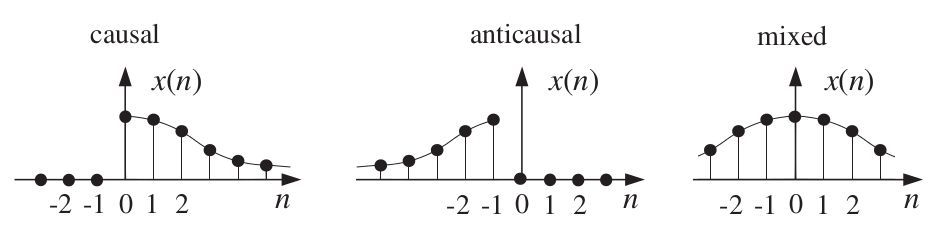
\includegraphics[width=15cm]{./picture/causality}

\subsection{Stability\buchSeite{115}}
\textbf{Stability Condition} $\sum\limits_{n=-\infty}^{\infty}\left| h(n)
\right| < \infty$\\
An LTI system is stable, if a bounded input can only generate bounded outputs.
Always prefer stability over causality!

\section{FIR Filtering and Convolution\buch{Chapter 4}}
\subsection{Block Processing Methods}
\subsubsection{Convolution}


\subsubsection{Direct Form}
\begin{tabular}{|l|l|}
	\hline
	$h$		& $h=[h_0,h_1, \ldots , h_M]$
	\\ \hline
	$L_h$	& $L_h = M + 1$
	\\ \hline
	$L_y$	& $L_y = L + M = L_x + L_h - 1$
	\\ \hline
	$y(n)$	& $y(n) = \sum\limits_{m=max(0,n-L+1)}^{min(n,M)} h(m)x(n-m)$
	\\ \hline 
\end{tabular}


\subsubsection{Convolution Table}

\begin{tikzpicture}
%lines
\draw (-0.5,3.5) -- (5.5, 3.5) -- (5.5,-0.5) -- (0.5,-0.5) -- (0.5,4.5);
\draw [dashed] (0.5,2) -- (2,3.5);
\draw [dashed] (0.5,1) -- (3,3.5);
\draw [dashed] (0.5,0) -- (4,3.5);
\draw [dashed] (1,-0.5) -- (5,3.5);
\draw [dashed] (2,-0.5) -- (5.5,3);
\draw [dashed] (3,-0.5) -- (5.5,2);
\draw [dashed] (4,-0.5) -- (5.5,1);

%nodes
\foreach \h in {0,1,2,3} {
	\node at (0,3-\h) {$h_{\h}$};
};
\foreach \x in {0,1,2,3,4} {
	\node at (\x+1, 4) {$x_{\x}$};
	\foreach \h in {0,1,2,3} {
		\node at (\x+1, 3-\h) {$h_{\h}x_{\x}$};
	};
};
\foreach \n in {0,...,5} {
	\node [rotate=45] at (\n+0.5,2.5) {$y_{\n}$};
};
\node [rotate=45] at (5.5,1.5) {$y_6$};
\node [rotate=45] at (5.5,0.5) {$y_7$};

\end{tikzpicture}

$y=[y_0, y_1, y_2, y_3, y_4, y_5, y_6, y_7]$


\subsubsection{LTI Form}
\begin{tabular}{c|cccccccc|}
	& $h_0$ & $h_1$ & $h_2$ & $h_3$ & 0 & 0 & 0 & 0 \\
	\hline
	$x_0$ & $x_0h_0$ & $x_0h_1$ & $x_0h_2$ & $x_0h_3$ & 0 & 0 & 0 & 0 \\
	$x_1$ & 0 & $x_1h_0$ & $x_1h_1$ & $x_1h_2$ & $x_1h_3$ & 0 & 0 & 0 \\
	$x_2$ & 0 & 0 & $x_2h_0$ & $x_2h_1$ & $x_2h_2$ & $x_2h_3$ & 0 & 0 \\
	$x_3$ & 0 & 0 & 0 & $x_3h_0$ & $x_3h_1$ & $x_3h_2$ & $x_3h_3$ & 0 \\
	$x_4$ & 0 & 0 & 0 & 0 & $x_4h_0$ & $x_4h_1$ & $x_4h_2$ & $x_4h_3$ \\
	\hline
	$y_n$ & $y_0$ & $y_1$ & $y_2$ & $y_3$ & $y_4$ & $y_5$ & $y_6$ & $y_7$ \\
\end{tabular}
\[
	y(n) = \sum\limits_{m=max(0,n-M)}^{min(n,L-1)} x(m)h(n-m)
\]


\subsubsection{Matrix Form}
The convolutional eqations can also be written in the linear matrix form:
\[
	y = H  x	\qquad \text{or} \qquad y = Xh
\]
where $H$ is built out of the filter's impulse response $h$ or the signal matrix $X$ is built out of the input signal. 
The filter matrix $H$, respectivly the signal matrix $X$, must be rectangular with dimensions
\[
	L_y \times L_x = (L + M)\times L \qquad \text{or} \qquad
	L_y \times L_h = (L + M)\times (M + 1)
\]

Example:
\setArrayStretch{1}
\[
	y =
	\begin{bmatrix}
		y_0 \\
		y_1 \\
		y_3 \\
		y_4 \\
		y_5 \\
		y_6 \\
		y_7
	\end{bmatrix}
	= \begin{bmatrix}
		h_0	& 0		& 0		& 0		& 0 \\
		h_1	& h_0	& 0 	& 0 	& 0 \\
		h_2	& h_1	& h_0	& 0		& 0 \\
		h_3 & h_2	& h_1	& h_0	& 0 \\
		0	& h_3	& h_2	& h_1	& h_0 \\
		0	& 0		& h_3	& h_2	& h_1 \\
		0	& 0		& 0		& h_3	& h_2 \\
		0	& 0		& 0		& 0		& h_3	 
	  \end{bmatrix}
	  \begin{bmatrix}
	  	x_0 \\
	  	x_1 \\
	  	x_2 \\
	  	x_3 \\
	  	x_4
	  \end{bmatrix}
	= Hx
\]
\resetArrayStretch


\subsubsection{Flip-and-Slide Form}
\begin{tikzpicture}

\foreach \h in {0,...,3} {
	\node at (3-\h,0) {$h_{\h}$};
	\node at (10-\h,0) {$h_{\h}$};
	\node at (15-\h,0) {$h_{\h}$};
	
};
\foreach \x in {0,...,2} {
	\node at (3+\x,-1) {$x_{\x}$};
};
\foreach \0 in {0,1,2,13,14,15} {
	\node at (\0,-1) {0};
};

\node at (6,-1) {$\cdot\cdot\cdot$};
\node at (7,-1) {$x_{n-3}$};
\node at (8,-1) {$x_{n-2}$};
\node at (9,-1) {$x_{n-1}$};
\node at (10,-1) {$x_{n}$};
\node at (11,-1) {$\cdot\cdot\cdot$};
\node at (12,-1) {$x_{L-1}$};

\draw (-0.3,0.3) rectangle (3.3,-0.3);
\draw (6.3,0.3) rectangle (10.3,-0.3);
\draw (11.3,0.3) rectangle (15.3,-0.3);
\draw (2.5,-0.7) rectangle (12.5,-1.3);
\draw [dashed] (-0.3,-1.3) rectangle (2.5,-0.7);
\draw [dashed] (15.3,-1.3) rectangle (12.5,-0.7);

\foreach \x in {0,1,2,3,7,8,9,10,12,13,14,15} {
	\draw (\x,-0.3) -- (\x,-0.7);
};

\draw [->] (3.3,0) -- (6.3,0);
\draw [->] (10.3,0) -- (11.3,0);
\foreach \x in {3,10,15} {
	\draw [->] (\x, -1.3) -- (\x,-1.7);
};

\node at (0,-1.5) [anchor=west] {M zeros};
\node at (13,-1.5) [anchor=west] {M zeros};

\node at (3,-2) {$y_0$};
\node at (10,-2) {$y_n$};
\node at (15,-2) {$y_{L-1+M}$};

\end{tikzpicture}
\[
	y(n) = h_0x_n + h_1x_{n-1}+\cdot\cdot\cdot+h_Mx_{n-M}
\]

\subsubsection{Overlap-Add Form}
\begin{enumerate}
  \item Divide input $x$ into smaller blocks $x_0, x_1, \ldots$ of length $L$.
  If the input is not long enough for a last complete block, the last block is
  filled up with zeroes
  \item Calculate the output of the convolution of block $x_0$ with $h$,
  resulting in $y_0$
  \item Repeat step 2 for all blocks, resulting in $y_1, y_2, \ldots$
  \item Add $y_0, y_1, \ldots$ up using the following table. $y_{n+1}$ is always
  moved to the right with an offset of $L$ compared to $y_n$.
\end{enumerate}

\begin{tabular}{c|ccccccccccc}
	n & 0 & 1 & 2 & 3 & 4 & 5 & 6 & 7 & 8 & 9 & 10 \\
	\hline
	$y_0$ & $y_{0,0}$ & $y_{0,1}$ & $y_{0,2}$ & $y_{0,3}$ & $y_{0,4}$ & $y_{0,5}$ &
	& & & &\\
	$y_1$ & & & & $y_{1,0}$ & $y_{1,1}$ & $y_{1,2}$ & $y_{1,3}$ & $y_{1,4}$ &
	$y_{1,5}$ & & \\
	$y_2$ & & & & & & & $y_{2,0}$ & $y_{2,1}$ & $y_{2,2}$ & $y_{2,3}$ & $y_{2,4}$
	\\
	\hline
\end{tabular}


\subsubsection{Transient and Steady-State Behavior}
\begin{tabular}{|l|l|}
	\hline
	input-on trainsients	& $ 0 \leq n < M $
	\\ \hline
	steady state			& $ M \leq n \leq L-1 $
	\\ \hline
	input-off transient		& $ L-1 < n \leq L-1+M $
	\\ \hline
\end{tabular}\newline

Therefore, the direct form takes the following different forms depending
on the value of the output index $n$:
\[
	y_n =
		\left\{
			\begin{array}{r l l l}
				\sum\limits_{m=0}^{n} & h_m x_{n-m}		& \quad \text{if } 0 \leq n < M			& \quad \text{input-on} \\
				\sum\limits_{m=0}^{M} & h_m x_{n-m}		& \quad \text{if } M \leq n \leq L-1	& \quad \text{steady state} \\
				\sum\limits_{m=n-L+1}^{M} & h_m x_{n-m}	& \quad \text{if } L-1 < n \leq L-1+M	& \quad \text{input-off}
			\end{array}
		\right.
\]


\subsubsection{Convolution of Infinite Sequences}
Three cases:
\setArrayStretch{1}
\begin{enumerate}
  \item Infinite filter, finite input; i.e., $M = \infty$, $L < \infty$
  \item Finite filter, infinite input; i.e., $M < \infty$, $L = \infty$
  \item Infinite filter, infinite input; i.e., $M = \infty$, $L = \infty$
\end{enumerate}
\resetArrayStretch

Therefore, the direct form takes the following different forms:
\[
	y_n =
		\left\{
			\begin{array}{r l l}
				\sum\limits_{m=max(0,n-L+1)}^{n} & h_m x_{n-m}		& \quad \text{if $M = \infty$, $L < \infty$} \\	
				\sum\limits_{m=0}^{min(n,M)} & h_m x_{n-m}		& \quad \text{if $M < \infty$, $L = \infty$ } \\
				\sum\limits_{m=0}^{n} & h_m x_{n-m}	& \quad \text{if $M = \infty$, $L = \infty$ }
			\end{array}
		\right.
\]




	
	
\section{z-Transformation\buch{Chapter 5}}

\subsection{Basic Properties\buchSeite{183}}

\[
	X(z) = \sum\limits_{n=-\infty}^\infty x(n)z^{-n}
\]

\begin{tabularx}{0.6\textwidth}{|l|r>{\centering}Xl|}
	\hline
	linearity & $a_1x_1(n) + a_2x_2(n)$ & $\overset{Z}{\longrightarrow}$ & $a_1X_1(z) + a_2X_2(z)$
	\\ \hline
	delay	& $x(n-D)$ & $\overset{Z}{\longrightarrow}$ & $z^{-D}X(z)$
	\\ \hline
	convolution & $y(n) = h(n) \convolution x(n)$ & $\overset{Z}{\longrightarrow}$ & $Y(z) = H(z)X(z)$
	\\ \hline
	modulation & $a^n g(n)$ & $\overset{Z}{\longrightarrow}$ & $G(\frac{z}{a})$
	\\ \hline
	time inversion & $g(-n)$ & $\overset{Z}{\longrightarrow}$ & $G(z^{-1})$
	\\ \hline
\end{tabularx}


\subsection{Region of Convergence (ROC)\buchSeite{186}}

\[
	\{ z \in \mathbb{C} \quad | \quad X(z) = \sum\limits_{n=-\infty}^{\infty} x(n)z^{-n} \neq \pm \infty \}
\]

\label{geometricseries}
\begin{tabular}{|l|l ll|}
	\hline
	infinite geometric series 1 & $1 + x + x^2 + x^3 + \ldots = \sum\limits_{n=0}^{\infty} x^n = \frac{1}{1-x}$ &&
	for $|x| < 1$
	\\ \hline
	infinite geometric series 2 & $x + x^2 + x^3 + \ldots = \sum\limits_{m=1}^{\infty} x^m = \frac{x}{1-x}$ &&
	for $|x| < 1$
	\\ \hline
\end{tabular}

If there is no ROC specified, we assume that the system is causal.


\subsection{Causality and Stability\buchSeite{193}}

For a signal or system to be simultaneously stable and \textbf{causal}, it is necessary that all its poles lie strictly 
\textbf{inside} the unit circle in the z-plane. 
\[ 1 > \max\limits_{i}|p_i| \]

A signal or system
can also be simultaneously stable and \textbf{anticausal}, but in this case all its poles must lie
strictly \textbf{outside} the unit circle.
\[ 1 < \min\limits_{i}|p_i| \]

\textbf{Marginally stable} signals have poles, that fall exactly onto the unit circle!

\subsection{Frequency Spectrum\buchSeite{196-210}}
\begin{multicols}{2}
	\begin{align}
	z=e^{j\omega} && \omega = \frac{2 \pi f}{f_s} \notag\\
	X(\omega)= \sum\limits_{n=-\infty}^{\infty} x(n)e^{-j\omega n} &&  \text{(DTFT)} \notag \\
	H(\omega)= \sum\limits_{n=-\infty}^{\infty} h(n)e^{-j\omega n} &&  \text{(frequency response)} \notag \\
	 -\pi \leq \omega \leq \pi && \text{nyquist interval}\notag\\
	x(n)= \frac{1}{2\pi} \int\limits_{-\pi}^{\pi} X(\omega)e^{j\omega n} d\omega &&\text{(inverse DTFT)} \notag
	\end{align}
\columnbreak
  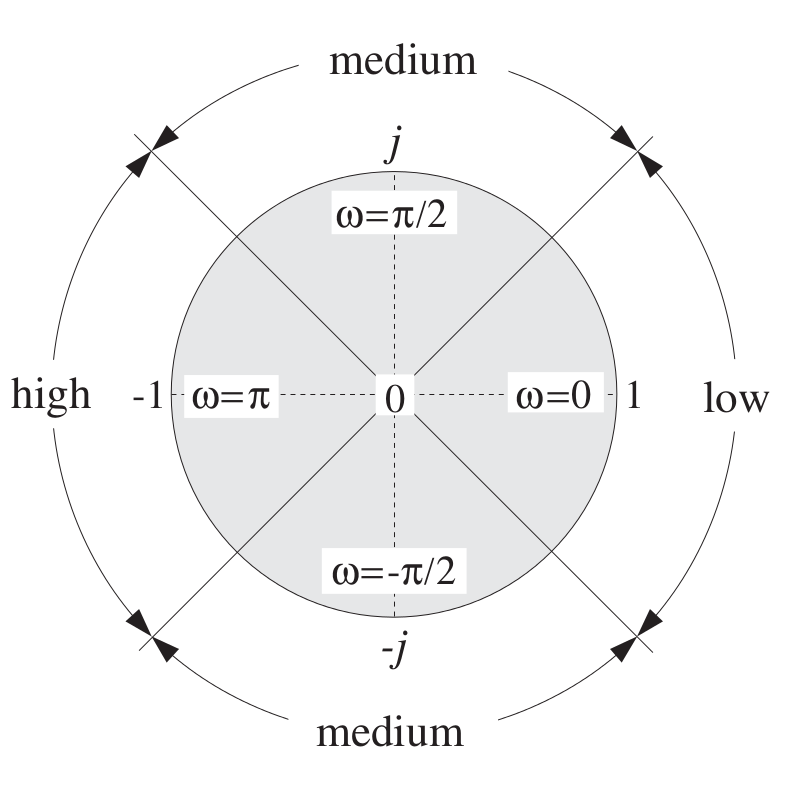
\includegraphics[width=6cm]{./picture/freq_spect}
\end{multicols}

Another useful relationship is Parseval’s equation, which relates the total energy of a sequence to its spectrum: 
\begin{align}
\sum_{n=-\infty}^{\infty} |x(n)|^2= \frac{1}{2\pi} \int\limits_{-\pi}^{\pi} |X(\omega)|^2 d\omega && \text{(Parseval)} \notag
\end{align}

Some DTFT-Transforms: \\ \\
\begin{tabularx}{0.7\textwidth}{|l|X|}
	\hline
	$\delta[n]$ &	$X_{2\pi}(\omega) = 1$ \\
	\hline 	
	$\delta[n-M]$ &	$X_{2\pi}(\omega) = e^{-i\omega M}$ \\
	\hline
	$u[n]$ & %$X_{2\pi}(\omega) = \frac{1}{1-e^{-i \omega}} + \pi \sum_{k=-\infty}^{\infty} \delta (\omega - 2\pi k) $ \\ & 	
	$X(\omega) = \frac{1}{1-e^{-i \omega}} + \pi \cdot \delta (\omega) $ \\
	\hline
	$e^{-i \omega_0 n}$ &	$X(\omega) = 2\pi\cdot \delta (\omega +\omega_0),     -\pi \leq \omega_0 < \pi$ \\
	\hline
	$\cos(\omega_0 n) $ & $X(\omega) = \pi [\delta (\omega +\omega_0)+\delta (\omega -\omega_0)],     -\pi < \omega_0 < \pi $\\
%	\\ & $X_{2\pi}(\omega) = \pi \sum_{k=-\infty}^{\infty} \left[ \delta (\omega - \omega_0 - 2\pi k) + 
%	\delta (\omega + \omega_0 + 2\pi k) \right] $ \\
	\hline
	$\sin(\omega_0 n) $ & $X(\omega) = -j \pi \delta(\omega - \omega_0) + j \pi \delta(\omega + \omega_0)$\\
%		$X_{2\pi}(\omega) = \frac{\pi}{i} \sum_{k=-\infty}^{\infty} \left[ \delta (\omega - \omega_0 - 2\pi k) 
%	- \delta ( \omega + \omega_0 + 2\pi k) \right] $  	\\
	\hline
\end{tabularx} \\ \\

\newpage

Some Z-Transforms:\\
\begin{tabularx}{0.6\textwidth}{|X|X|X|}
	\hline
	\textbf{x(n} ) & \textbf{X(z}) & \textbf{ROC} \\
	\hline
	$u(n)$ & $\frac{1}{1 - z^{-1}}$ & $|z|>1$ \\
	\hline
	$-u(-n-1)$ & $\frac{1}{1 - z^{-1}}$ & $|z|<1$ \\
	\hline
	$(-1)^n u(n)$ & $\frac{1}{1 + z^{-1}}$ & $|z|>1$ \\
	\hline
	$-(-1)^n u(-n-1)$ & $\frac{1}{1 + z^{-1}}$ & $|z|<1$ \\
	\hline
	$a^n u(n)$ & $\frac{1}{1 - az^{-1}}$ & $|z|>|a| \quad$ (causal) \\
	\hline
	$-a^n u(-n-1)$ & $\frac{1}{1 - az^{-1}}$ & $|z|<|a| \quad$ (acausal) \\
	\hline
	$e^{\alpha n}$ & $\frac{z}{z-e^{\alpha}}$ & \\
	\hline
	$\cos(\omega n)$ & $\frac{z(z-\cos(\omega))}{z^2 -2z\cos(\omega) + 1}$ & \\
	\hline
	$\sin(\omega n)$ & $\frac{z\sin(\omega)}{z^2 -2z\cos(\omega) + 1}$ & \\
	\hline
	$A\delta(n)$ & $A$ & \\
	\hline
\end{tabularx}
\begin{minipage}[b][5.4cm][t]{5cm}
	For real valued discrete time sequences:\\
	$X(\omega)^* = X(-\omega)$ \\
	$|X(\omega)| = |X(\omega)|$\\
	$argX(\omega) = -argX(-\omega)$
\end{minipage}


\subsection{Inverse z-Transforms\buchSeite{202-204}}

$X(z) = \dfrac{N(z)}{D(z)} = \dfrac{N(z)}{(1-p_1z^{-1})(1-p_2z^{-1})\ldots(1-p_Mz^{-1})} = 
A_0 + \dfrac{A_1}{1-p_1z^{-1}} + \ldots + \dfrac{A_M}{1-p_Mz^{-1}}$

with $A_0 = X(z)|_{z=0}$ \\

\textbf{PBZ\buchSeite{203}:} for Order of $N(z) <$ Order of $D(z)$ \\
\[A_i = [(1-p_iz^{-1})X(z)]_{z=p_i} = \left[\frac{N(z)}{\prod\limits_{j\neq i}(1-p_jz^{-1})}\right]_{z=p_i}\]

\textbf{Euler:}

\begin{align}
\cos(\alpha) = \frac{e^{j\alpha} + e^{-j\alpha}}{2}
&& \sin(\alpha) = \frac{e^{j\alpha} - e^{-j\alpha}}{2j} && 
    {e}^{\pm jn\omega} = \cos{n\omega} \pm j \sin{n\omega} \notag\\
e^{j\frac{\pi}{2}n} = j^n & & e^{-j\frac{\pi}{2}n} = (-j)^n &&
e^{jn\pi}=e^{-jn\pi}=(-1)^n \notag
\end{align}
$(1-ae^{j\omega}z^{-1})(1-ae^{-j\omega}z^{-1}) = 1 - 2a\cos(\omega)z^{-1}+a^2z^{-2}$



\section{Transfer Functions\buch{Chapter 6}}
\subsection{IIR-Form:\buchSeite{223,224}}
\begin{align}
H(z) = \frac{N(z)}{D(z)}
		= \frac{b_0 + b_1 z^{-1} + b_2 z^{-2} + \ldots + b_N z^{-N}}{1 + a_1 z^{-1} + a_2 z^{-2} + \ldots + a_M z^{-M} } && a_0 = 1 \text{ normalize to } 1 \notag
\end{align}

if $D(z) = 1$, the IIR Form can be reduced to a FIR Filter:
\[
	H(z) = N(z) = b_0 + b_1 z^{-1} + b_2 z^{-2} + \ldots + b_N z^{-N}
\]

Example: find $H(z)$ for $h(n) = \left[1,3,4,5\right]$
\[ H(z) = 1 + 3z^{-1} + 4z^{-2} + 5z^{-3}\]

Example: $y(n) = 0.25 \cdot y(n-2) + x(n) $
\[
	Y(z) = 0.25z^{-2}Y(z) + X(z)
\]

\subsection{Steady state response\buchSeite{230-232}}
\[\cos(\omega_0 n) \rightarrow \left|H(\omega_0) \right| \cos(\omega_0 n + \arg(H(\omega_0))) \]

\[\sin(\omega_0 n) \rightarrow \left|H(\omega_0) \right| \sin(\omega_0 n + \arg(H(\omega_0))) \]

\begin{tabularx}{0.6\textwidth}{|l|X|}
	\hline
	phase delay & $d(\omega) = - \frac{\arg(H(\omega))}{\omega}$\ \qquad $\arg H(\omega = -\omega d(\omega))$
	\\ \hline 
	group delay & $d_g(\omega) = -\frac{d}{d\omega}(\arg(H(\omega)))$	
	\\ \hline
\end{tabularx}\\ \\

\subsection{Transient Response\buchSeite{232}}
\begin{align}
&\text{complex sinuousness:} & & x(n) = e^{j \omega_0 n} \cdot u(n) && \Rightarrow && X(Z) = \frac{1}{1-e^{j \omega_0} z^{-1}} && ROC |z| > |e^{j\omega_0}|=1\notag\\ 
&\text{effective time:} && n_{eff} = \frac{\ln \epsilon}{\ln \rho} &&\text{with: }& &\rho = \max\limits_{i}\left|p_i \right| &&\notag\\
&\text{f and magnitude reponses:} && H(\omega)=\frac{b}{1-ae^{-j\omega}} &&\Rightarrow &&
\left| H(\omega)\right| = \frac{b}{\sqrt{1-2a\cos(\omega) + a^2}} &&\notag\\
&\text{requirement that:} && |H(\omega_0)|=1 &&&& &&\notag
\end{align}\\
$\left| 1-a e^{-j\omega}\right| = \sqrt{1-2a\cos(\omega) + a^2}$\\

\subsection{Unit Step Response\buchSeite{239}}
\begin{tabularx}{1\textwidth}{l X}
	DC-Gain: & $H(0) = H(z)|_{z=1}= \sum\limits_{n=0}^{\infty}h(n) $
	\\
	AC-Gain: & $H(\pi) = H(z)|_{z=-1}= \sum\limits_{n=0}^{\infty}(-1)^n h(n) $
\end{tabularx}\\ \\


\subsection{Pole/Zero Design\buchSeite{242,245}}
\begin{tabularx}{1\textwidth}{Xll}
	3dB width & $\Delta\omega \simeq 2(1-R)$ & $=:R$ is the pole \\
	full width at half maximum of the magnitude squared response & $|H(\omega)|^2=\frac{1}{2}|H(\omega_0)|^2=\frac{1}{2}$&
\end{tabularx}\\ \\

\subsubsection{2 pole conjugate filter\buchSeite{244-246}}

\begin{tabularx}{1\textwidth}{l X}
	poles: & $ p = R e^{j\omega}$ \qquad and \qquad $ p^* = R e^{-j\omega}$
	\\ 
	Transfer function: & $H(z)= \frac{G}{(1-R e^{-j\omega}z^{-1})(1-Re^{j\omega}z^{-1})}$\
	$=\frac{G}{1+a_1z^{-1}+a_2z^{-2}}$
	\\
	Parameter: & $a_1 = -2R\cos(\omega_0)$ \qquad; \qquad $a_2 = R^2$
	\\ 
	filter impulse Response & $h(n) = \frac{G}{\sin(\omega_0)}R^n \sin(\omega_0 n + \omega_0)$
	\\ 
	& $G = (1-R)\sqrt{1-2R\cos(2\omega_0)+ R^2}$
\end{tabularx}\\ \\

\subsubsection{2 pole 2 zero filter\buchSeite{228,249}}

\begin{tabularx}{1\textwidth}{l X}
	poles: & $ p = R e^{j\omega}$ \qquad and \qquad $ p^* = R e^{-j\omega}$
	\\ 
	zeros: & $ z_1 = r e^{j\omega}$ \qquad and \qquad $ z_1^* = r e^{-j\omega}$
	\\
	Transfer function: & $H(z)= \frac{(1-r e^{j\omega}z^{-1})(1-re^{-j\omega}z^{-1})}{(1-R e^{j\omega}z^{-1})(1-Re^{-j\omega}z^{-1})}$\
	$=\frac{1+b_1z^{-1}+b_2z^{-2}}{1+a_1z^{-1}+a_2z^{-2}}$
	\\ 
	Parameter: & $a_1 = -2R\cos(\omega_0)$ \qquad; \qquad $a_2 = R^2$
	\\ 
	& $b_1 = -2r\cos(\omega_0)$ \qquad; \qquad $b_2 = r^2$
\end{tabularx}\\ \\

\subsubsection{Notch and Comb Filter\buchSeite{249-251}}
The zeros of the filters located on the unit circle and the poles are in the unit
circle.

\begin{tabularx}{1\textwidth}{l X}
	Transfer function: & $H(z) = \frac{N(z)}{D(z)} $
	\\
	& $N(z) = \prod\limits_{i=1}^{M}(1- e^{j\omega_i}z^{-1)} $ \qquad (notch polynomial)
	\\
	& $D(z) = N(\rho^{-1})  = \prod\limits_{i=1}^{M}(1- e^{j\omega_i}\rho z^{-1)} $
	\\
	& $H(z) = \frac{N(z)}{(N\rho^{-1}z)}= \frac{1+b_1 z^{-1} + b_2z^{-2} + \ldots + b_M z^{-M}}
	{1+\rho b_1 z^{-1} + \rho^2 b_2z^{-2} + \ldots + \rho^M b_M z^{-M}} $\\
	&$a_i=\rho^ib_i \qquad$ mit $\qquad i=1,2,\ldots,M$ \\
	\end{tabularx}\\ \\



\end{document}
 